\documentclass{exercise}

\institute{Lehr- und Forschungsgebiet Kontinuumsmechanik}
\title{Übung 5}
\author{Joshua Feld, 406718}
\course{Mechanik verformbarer Körper}
\professor{Itskov}
\semester{Sommersemester 2022}
\program{CES (Bachelor)}

\begin{document}
    \maketitle


    \section*{Aufgabe 1}

    \begin{problem}
        \begin{minipage}{.75\textwidth}
            Eine elastische Stütze (Elastizitätsmodul \(E\)) der Länge \(l\) ist in \(B\) und \(C\) gelenkig gelagert und im unbelasteten Zustand spannungsfrei.
            Sie wird in \(D\) mit einer Einzelkraft \(F\) belastet, die als gleichmäßig über dem Querschnitt \(A\) verteilt angenommen wird.
            \begin{enumerate}
                \item Berechnen Sie die Spannungen in den Abschnitten \(1\) und \(2\).
                \item Berechnen Sie die Verschiebung des Kraftangriffpunktes \(D\).
            \end{enumerate}
            Gegeben: \(a\), \(l\), \(A\), \(F\), \(E\)
        \end{minipage}
        \begin{minipage}{.25\textwidth}
            \begin{flushright}
                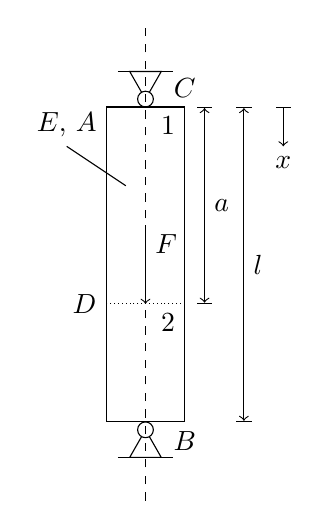
\begin{tikzpicture}
                    \draw (.3,-.45) -- (.5,-.1) -- (.7,-.45) -- cycle;
                    \draw (.15,-.45) -- (.85,-.45);
                    \draw[fill=white] (.5,-.1) circle (1mm);
                    \draw (.3,4.45) -- (.5,4.1) -- (.7,4.45) -- cycle;
                    \draw (.15,4.45) -- (.85,4.45);
                    \draw[fill=white] (.5,4.1) circle (1mm);
                    \draw (0,0) rectangle (1,4);
                    \node[anchor=north] at (1,0) {\(B\)};
                    \node[anchor=south] at (1,4) {\(C\)};
                    \draw[densely dotted] (1,1.5) -- (0,1.5) node[left] {\(D\)};
                    \draw[dashed] (.5,-1) -- (.5,5);
                    \draw[|->] (2.25,4) -- (2.25,3.5) node[below] {\(x\)};
                    \draw[|<->|] (1.25,4) -- (1.25,1.5) node[midway,right] {\(a\)};
                    \draw[|<->|] (1.75,4) -- (1.75,0) node[midway,right] {\(l\)};
                    \node[anchor=north east] at (1,4) {\(1\)};
                    \node[anchor=north east] at (1,1.5) {\(2\)};
                    \draw[->] (.5,2.5) node[below right] {\(F\)} -- (.5,1.5);
                    \draw (.25,3) -- (-.5,3.5) node[above] {\(E\), \(A\)};
                \end{tikzpicture}
            \end{flushright}
        \end{minipage}
    \end{problem}

    \subsection*{Lösung}
    \begin{enumerate}
        \item Das Kräftegleichgewicht in \(\downarrow\)-Richtung im Kraftangriffspunkt \(D\) lautet
        \[
            -F_1 + F_2 + F = 0.
        \]
        Mit der Längenänderung der beiden Einzelteile
        \[
            \Delta l_1 = \frac{F_1 l_1}{EA}, \quad \Delta l_2 = \frac{F_2 l_2}{EA}
        \]
        und der Verträglichkeitsbedingung
        \[
            \Delta l = \Delta l_1 + \Delta l_2 = 0
        \]
        folgt
        \[
            F_1 l_1 = -F_2 l_2 \implies F_1 a = -F_2\parentheses*{l - a}
        \]
        und somit folgt aus dem Kräftegleichgewicht
        \[
            F_2\frac{l - a}{a} + F_2 + F = 0
        \]
        für die Kräfte in den Einzelteilen
        \[
            F_2 = -\frac{Fa}{l}, \quad F_1 = \frac{F\parentheses*{l - a}}{l}.
        \]
        Die Spannungen ergeben sich zu
        \[
            \sigma_2 = -\frac{Fa}{Al}, \quad \sigma_1 = \frac{F\parentheses*{l - a}}{Al}.
        \]
        \item Die Verschiebung des Kraftangriffspunktes entspricht der Längenänderung des oberen Bauteils
        \[
            \Delta l_1 = \frac{F_1 l_1}{EA} = \frac{\frac{F\parentheses*{l - a}}{l}a}{EA} = \frac{F\parentheses*{l - a}a}{EAl}.
        \]
    \end{enumerate}


    \section*{Aufgabe 2}

    \begin{problem}
        Ein Stahlstab mit kreisförmigen Querschnitt hat einen konstanten Durchmesser von \(d\) und die Länge \(l\).
        Er ist bei einer Temperatur von \(T_0\) spannungsfrei zwischen zwei Wänden gelagert.
        \begin{enumerate}
            \item Berechnen Sie die Spannungen für den Fall, dass der unlösbar mit den Wänden verbundene Stab auf \(T_1\) abgekühlt wird.
            Wie groß ist die auf die Wände wirkende Kraft?
            \item Berechnen Sie die Verformung des Stabes für den Fall, dass der Stab nur an einer Wand fixiert ist.
        \end{enumerate}
        Gegeben: \(d = 5\sis{\milli\meter}\), \(l = 1000\sis{\milli\meter}\), \(T_0 = 20\si{\degreeCelsius}\), \(T_1 = 10\si{\degreeCelsius}\), \(E = 2,1 \cdot 10^5\sis{\newton\per\milli\meter\squared}\), \(\alpha_T = 12 \cdot 10^{-6}\sis{\per\kelvin}\)
    \end{problem}

    \subsection*{Lösung}
    Die Wärmedehnung \(\varepsilon_T\) sei proportional zur Temperaturdifferenz \(\Delta T\) mit dem Proportionalitätsfaktor \(\alpha_T\)
    \[
        \varepsilon_T = \alpha_T \Delta T.
    \]
    \(\alpha_T\) heißt thermischer Ausdehnungskoeffizient oder Wärmeausdehnungskoeffizient (Einheit \(\si{\per\kelvin}\)).
    Der Stabquerschnitt ergibt sich zu \(A = \frac{\pi d^2}{4}\).
    Die Temperaturänderung ist \(\Delta T = T_1 - T_0 = -10\si{\degreeCelsius}\).
    \begin{enumerate}
        \item Aufgrund der festen Einspannung gilt \(\Delta l = 0 \implies \varepsilon_x = 0\).
        Das Hook'sche Gesetz in verallgemeinerter Form
        \[
            \varepsilon_x = \frac{1}{E}\parentheses*{\sigma_x - \nu\parentheses*{\sigma_y + \sigma_z}} + \alpha_T \Delta T
        \]
        liefert (mit \(\sigma_y = \sigma_z = 0\))
        \[
            \sigma_x = -E\alpha_T \Delta T = 25,2\sis{\newton\per\milli\meter\squared}.
        \]
        Für die Kraft folgt
        \[
            F_x = \sigma_x A = 494,8\sis{\newton}.
        \]
        \item Für das lose Ende gilt \(\sigma_x = 0\).
        Das Hook'sche Gesetz in verallgemeinerter Form
        \[
            \varepsilon_x = \frac{1}{E}\parentheses*{\sigma_x - \nu\parentheses*{\sigma_y + \sigma_z}} + \alpha_T \Delta T
        \]
        liefert (mit \(\sigma_x = \sigma_y = \sigma_z = 0\))
        \[
            \varepsilon_x = \alpha_T \Delta T = -1,2 \cdot 10^{-4}.
        \]
        Für die Längenänderung ergibt sich
        \[
            \Delta l = \varepsilon_x l = -0,12\sis{\milli\meter}.
        \]
    \end{enumerate}


    \section*{Aufgabe 3}

    \begin{problem}
        Ein abgesetztes Bauteil wird um \(\Delta T\) erwärmt.
        \begin{enumerate}
            \item Bei welcher Temperaturänderung \(\Delta T\) berührt das Bauteil die Wand?
            \item Wie groß sind die Spannungen in den Abschnitten \(1\) und \(2\) sowie die Verschiebung des Punktes \(C\), wenn das Bauteil um \(\Delta T = 40\sis{\kelvin}\) erwärmt wird?
        \end{enumerate}
        Gegeben: \(l_1 = 2\sis{\meter}\), \(l_2 = 1,5\sis{\meter}\), \(A_1 = 800\sis{\milli\meter\squared}\), \(A_2 = 700\sis{\milli\meter\squared}\), \(E = 2,1 \cdot 10^5\sis{\newton\per\milli\meter\squared}\), \(\alpha = 12 \cdot 10^{-6}\sis{\per\kelvin}\), \(\delta = 1,2\sis{\milli\meter}\), \(\Delta T = 40\sis{\kelvin}\)
    \end{problem}

    \subsection*{Lösung}
    \begin{enumerate}
        \item Bis zu einer Verlängerung um \(\delta\) kann sich das Bauteil ungehindert ausdehnen.
        Es gilt \(\delta = \Delta l_1 + \Delta l_2 = 1,2\sis{\milli\meter}\) und \(\sigma_1 = \sigma_2 = 0\).
        Mit den Hook'schen Gesetz folgt
        \[
            \Delta l_1 = l_1\alpha\Delta T, \quad \Delta l_2 = l_2\alpha\Delta T.
        \]
        Somit gilt
        \[
            \delta = \alpha\Delta T\parentheses*{l_1 + l_2} \implies \Delta T = \frac{\delta}{\alpha\parentheses*{l_1 + l_2}} = 28,57\sis{\kelvin}.
        \]
        \item Bei einer Erhöhung der Temperatur um mehr als \(28,57\sis{\kelvin}\) wird die weitere Ausdehnung verhindert und die einzelnen Bauteile sind nicht mehr spannungsfrei.
        Es gilt \(\delta = \Delta l_1 + \Delta l_2 = 1,2\sis{\milli\meter}\) und aufgrund des Kräftegleichgewichts zwischen den beiden Teilen \(F_1 = \sigma_1 A_1 = \sigma_2 A_2 = F_2\).
        Mit dem Hook'schen Gesetz
        \[
            \Delta l = \frac{Fl_0}{EA} + \alpha\Delta Tl_0
        \]
        folgt
        \[
            \delta = \Delta l_1 + \Delta l_2 = F\parentheses*{\frac{l_1}{EA_1} + \frac{l_2}{EA_2}} + \alpha\Delta T\parentheses*{l_1 + l_2}
        \]
        und somit
        \[
            F = -2,17 \cdot 10^4\sis{\newton}.
        \]
        Für die Spannungen folgt
        \[
            \sigma_1 = \frac{F}{A_1} = -27,14\sis{\newton\per\milli\meter\squared}, \quad \sigma_2 = \frac{F}{A_2} = -31,01\sis{\newton\per\milli\meter\squared}.
        \]
        Die Verschiebung des Punktes \(C\) ist gleich der Längenänderung
        \[
            \Delta l_1 = \frac{Fl_1}{EA_1} + \alpha\Delta Tl_1 = 0,702\sis{\milli\meter}.
        \]
    \end{enumerate}


    \section*{Aufgabe 4}

    \begin{problem}
        Ein konischer Stab der Länge \(L\) mit kreisförmigen Querschnitt (Durchmesser \(D_0 \le D \le D_L, D_L \ll L\)) liegt spiel- und spannungsfrei zwischen zwei starren Wänden.
        Der Stab besteht aus einem homogenen, linear-elastischen Material (Elastizitätsmodul \(E\), Wärmeübergangskoeffizient \(\alpha\)) und wird gleichmäßig um eine Temperatur \(\Delta \vartheta\) erwärmt.
        \begin{enumerate}
            \item Wie groß ist die in dem Stab auftretende maximale Spannung?
            \item Wie groß ist das Verhältnis der Spannungen an den Enden des Stabes?
        \end{enumerate}
        Gegeben: \(D_0\), \(D_L\), \(L\), \(E\), \(\alpha\), \(\Delta\vartheta\)
    \end{problem}

    \subsection*{Lösung}
    \begin{enumerate}
        \item Das Hook'sche Gesetz in Abhängigkeit von \(x\) (\(0 \le x \le L\)) lautet
        \[
            \varepsilon\parentheses*{x} = \frac{F}{A\parentheses*{x}E} + \alpha\Delta\vartheta
        \]
        mit der veränderlichen Querschnittsfläche
        \[
            A\parentheses*{x} = \frac{\pi}{4}\parentheses*{D_0 + \frac{D_L - D_0}{L}x}^2.
        \]
        Für die Verschiebung gilt
        \[
            u = \int\varepsilon\parentheses*{x}\d x
        \]
        und somit folgt für die Längenänderung
        \[
            \Delta L = \int_0^L \varepsilon\parentheses*{x}\d x = \int_0^L \parentheses*{\frac{4F}{\pi E}\parentheses*{D_0 + \frac{D_L - D_0}{L}x}^{-2} + \alpha\Delta\vartheta}\d x.
        \]
        Mit der Substitution
        \[
            w = D_0 + \frac{D_L - D_0}{L}x \implies \frac{\d w}{\d x} = \frac{D_L - D_0}{L} \implies \d x = \frac{L}{D_L - D_0}\d w
        \]
        lässt sich der Ausdruck zu
        \[
            \Delta L = \frac{L}{D_L - D_0}\int_{D_0}^{D_L}\parentheses*{\frac{4F}{\pi E}w^{-2} + \alpha\Delta\vartheta}\d w
        \]
        umschreiben.
        Integriert folgt
        \[
            \Delta L = \frac{L}{D_L - D_0}\brackets*{-\frac{4F}{\pi E}w^{-1} + \alpha\Delta\vartheta w}_{D_0}^{D_L} = \frac{4FL}{\pi ED_0 D_L} + \alpha\Delta\vartheta L.
        \]
        Da der Stab eingespannt ist und keine Längenänderung erfolgen kann, gilt \(\Delta L = 0\) und für die konstante Kraft \(F\) folgt
        \[
            F = -\frac{\alpha\Delta\vartheta\pi ED_L D_0}{4}.
        \]
        Für die Spannung gilt der Zusammenhang
        \[
            \sigma\parentheses*{x} = \frac{F\parentheses*{x}}{A\parentheses*{x}} = \frac{F}{A\parentheses*{x}},
        \]
        somit ist die Spannung dort am größten, wo die Querschnittsfläche am kleinsten ist:
        \[
            \sigma_{\text{max}} = \sigma\parentheses*{0} = \frac{F}{A\parentheses*{0}} = -\frac{\alpha\Delta\vartheta ED_L}{D_0}.
        \]
        \item
        \[
            \frac{\sigma\parentheses*{0}}{\sigma\parentheses*{L}} = \frac{\frac{F}{A\parentheses*{0}}}{\frac{F}{A\parentheses*{L}}} = \frac{A\parentheses*{L}}{A\parentheses*{0}} = \frac{D_L^2}{D_0^2}.
        \]
    \end{enumerate}


    \section*{Aufgabe 5}

    \begin{problem}
        Einige Studenten haben vor, die Beschaffenheit des Bodens unter der RWTH geologisch zu erkunden.
        Zu diesem Zweck haben sie ein Bohrgestänge konstruiert, mit dem sie in die Tiefe \(t\) vordringen.
        Das Bohrgestänge besteht aus gleichartigen Stahlrohren.
        Wie groß ist die Längenänderung des Bohrgestänges aufgrund des Eigengewichtes?

        Gegeben: \(t = 6000\sis{\meter}\), \(\rho = 7,86 \cdot 10^3\sis{\kilo\gram\per\meter\cubed}\), \(g = 9,81\sis{\meter\per\second\squared}\), \(E = 2,1 \cdot 10^5\sis{\newton\per\milli\meter\squared}\)
    \end{problem}

    \subsection*{Lösung}
    Es wird angenommen, dass sich die Fallbeschleunigung \(g\) nicht über die Tiefe des Lochs ändert.
    Dies ist gerechtfertigt, da der Radius der Erde ca. \(1000\)-fach größer ist als die Tiefe des Lochs.
    Weiterhin wird angenommen, dass das Bohrgestänge ausschließlich am oberen Ende (Turm) eingespannt ist.

    Die Dehnung der Stange ist nicht konstant.
    Am unteren Ende der Stange ist sie gleich Null, am oberen Ende maximal.
    Die Verschiebung ist in der Einspannung (oben) Null und unten im Loch maximal.
    Wir definieren das obere Ende der Stange als \(z = 0\) und das untere Ende der Stange als \(z = t = 6000\sis{\meter}\).

    Für die aufgrund der Gravitation wirkenden Kraft ergibt sich
    \[
        F\parentheses*{z} = mg = \rho Vg = \rho A\parentheses*{t - z}g.
    \]
    Für die Kraft aufgrund der Gravitation in einer bestimmten Tiefe \(z\) spielt nur das Gewicht des darunter liegenden Teils des Gestänges eine Rolle.
    \(m\) bezeichnet hierbei die Masse, \(V\) das Volumen und \(A\) den Querschnitt dieses Gestängeteils.
    Des Weiteren gelten die Beziehungen
    \[
        \sigma\parentheses*{z} = \frac{F\parentheses*{z}}{A}, \quad \varepsilon\parentheses*{z} = \frac{\sigma\parentheses*{z}}{E}, \quad \Delta l = \int\varepsilon\parentheses*{z}.
    \]
    Für die Dehnung in der Tiefe \(z\) folgt somit
    \[
        \varepsilon\parentheses*{z} = \frac{\rho\parentheses*{t - z}g}{E}
    \]
    und für die gesamte Längenänderung über die komplette Tiefe \(t\) gilt daher
    \[
        \Delta l = \int_0^t \varepsilon\parentheses*{z}\d z = \frac{\rho gt^2}{2E} = 6,61\sis{\meter}.
    \]
\end{document}
